\documentclass{article}


\usepackage{PRIMEarxiv}

\usepackage[utf8]{inputenc} % allow utf-8 input
\usepackage[T1]{fontenc}    % use 8-bit T1 fonts
\usepackage{hyperref}       % hyperlinks
\usepackage{url}            % simple URL typesetting
\usepackage{booktabs}       % professional-quality tables
\usepackage{amsfonts}       % blackboard math symbols
\usepackage{nicefrac}       % compact symbols for 1/2, etc.
\usepackage{microtype}      % microtypography
\usepackage{lipsum}
\usepackage{fancyhdr}       % header
\usepackage{graphicx}       % graphics
\graphicspath{{media/}}     % organize your images and other figures under media/ folder
\usepackage{amsmath}

%Header
\pagestyle{fancy}
\thispagestyle{empty}
\rhead{ \textit{ }} 

% Update your Headers here
\fancyhead[LO]{Tiling Spaces and the Expanding Universe}

  
%% Title
\title{Tiling Spaces and the Expanding Universe: Bridging Quantum Mechanics and Cosmology}

\author{Aman Yadav\textsuperscript{1} and Marcelo Maciel Amaral,\textsuperscript{2}\\
  \textsuperscript{1}\emph{Department of Civil Engineering, Delhi
Technological University, Delhi 110042, India}\\
\textsuperscript{2}\emph{Quantum Gravity Research, Los Angeles, CA 90290, USA}\\
Correspondence: \texttt{amanyadaav11@gmail.com}\\
}



\begin{document}
\maketitle


\begin{abstract}
We propose a heuristic model of the universe as a growing quasicrystal projected from a higher-dimensional lattice. By extending the Schr{\"o}dinger equation for a particle in a box with time-dependent boundaries, we derive an equation that resembles the Friedmann equation, addressing the Hubble tension. This model incorporates phonons and phasons, providing insights into cosmic-scale dynamics and the universe’s expansion. We outline a pre-inflation tiling space phase with quantum error correction, a radiation phase dominated by quasiparticles, and a post-radiation phase with the emergence of matter. Our hypothesis, which posits that the universe is a growing quasicrystal, suggests that the necessity for an inflationary period may be obviated. Furthermore, phonon arising from this quasicrystalline structure could act as dark matter, influencing the dynamics of ordinary matter while remaining mostly undetectable by electromagnetic interactions. This hypothesis draws parallels with other crystalline matters at atomic scales that are fundamentally quantum in nature. We also explore how the notion of tiling space can support continuous symmetry atop a discrete structure, providing a novel framework for understanding the universe’s expansion and underlying structure. Consequently, it is logical to start with quantum mechanics as the foundation of our model. Further development could enhance our understanding of cosmic expansion and the underlying structure of the universe.
\end{abstract}




% keywords can be removed
\keywords{Quantum Gravity \and Cosmology \and Hubble Tension \and Quasicrystals}

\tableofcontents

\section{Introduction}
\label{intro}

Recent developments in theoretical physics have propelled us toward a deeper understanding of spacetime and gravity. The field of emergent gravity \cite{Verlinde2011} suggests that spacetime and gravity might be the byproducts of fundamental quantum mechanical processes. This paradigm shift is supported by theories such as loop quantum gravity and spin foam \cite{Rovelli-Vidotto-Book}, as well as superstring theory and M theory \cite{stringbook1}, all of which propose a quantum-level discreteness underlying gravity.

A key focus since the advent of perturbative superstring theory has been the quest to unravel quantum gravity \cite{Kiefer}. This endeavor involves comprehending the theory's foundational principles and extracting insights about Planck-scale physics \cite{Rovelli1998}. Consequently, there is a growing trend to incorporate concepts from condensed matter or solid-state physics, such as viewing spacetime as a deformable solid or crystal \cite{Tahim2009}. More recently, quasicrystals have been investigated \cite{Amaral:2023mgf,modelsetemergence}.


Clues that our theories about reality are incomplete are emerging in various fields, from anomalies in particle physics experiments to unresolved problems in cosmology \cite{lawsofnature}. For instance, the discovery of neutrino oscillations challenged the Standard Model of particle physics, indicating that neutrinos have mass. Similarly, in cosmology, the Hubble tension \cite{hubbletension} represents a profound discrepancy between measurements of the universe's expansion rate. On one side, observations of the Cosmic Microwave Background (CMB) by missions like the European Space Agency's Planck satellite suggest a slower expansion rate, based on the state of the universe shortly after the Big Bang and theoretical models of its evolution—around 67-68 km/s/Mpc. On the other, direct measurements of the current universe, notably from the Hubble Space Telescope and confirmed by the James Webb Space Telescope, indicate a significantly faster rate \cite{hubble}—around 73-74 km/s/Mpc. This tension challenges our understanding of the cosmos and suggests that our theoretical models of the universe may be incomplete, indicating that new physics might be necessary to resolve the discrepancy. Despite the increased precision of observational instruments and techniques, this persistent tension highlights a crucial gap in our understanding of fundamental cosmic processes, making it a focal point for theoretical and observational cosmology alike.


Our research adopts a dual approach within this context. First, we start with conventional quantum mechanics. While the universe's expansion is typically addressed from a classical perspective on large scales, this expansion must also extend down to microscopic scales, as suggested by various approaches to quantum cosmology \cite{bojowald,Kuzmichev}. Unlike conventional quantum cosmology, we analyze the wave function of a particle with mass $m$ in a specific spatial domain using the Schr{\"o}dinger equation, thereby focusing on intermediate scales. Crucially, we posit that the wavenumber, wavelength, and quantum amplitudes become functions of the dynamical size of the box and are subject to the Hubble law explicitly. Considerations about the dynamic boundary of the spatial domain lead us to a version of the Friedmann equation, crucial in cosmological models, thereby underscoring the emergence of classical spacetime from quantum mechanics. 

Second, drawing inspiration from the concept of a deformable solid or crystal and quantum cosmology, which deals with discreteness, we propose modeling spacetime as a growing quasicrystal. Characterized by long-range order without periodicity, this structure reflects the aperiodic patterns found in condensed matter physics. Our principal finding suggests that the cosmological scale factor might be interpreted as an inherent scaling characteristic within a quasicrystal tiling space framework. We also consider the implications of this model for the Hubble tension, offering a fresh perspective on the general evolution of the universe and providing new insights into other issues in current cosmology models, such as dark matter and dark energy.

Our research adopts a dual approach that intersects at the idea of rescaling the underlying geometry, accompanied by emerging constraints pertinent to physics at varying scales. This approach aligns with our methodology of conceptualizing spacetime through the lens of a quasicrystalline structure. By integrating scale invariance into our framework, we aim to forge a connection between the microscale realms of quantum mechanics and the macroscale phenomena observed in cosmology. This synthesis offers a comprehensive and unified perspective, potentially enhancing our understanding of the universe's nature.

In the following sections, we will further elaborate on the mathematical foundations of our model, exploring how energy considerations translate into cosmological parameters. Moreover, we will delve into the concept of spacetime as a tiling space, drawing parallels with quasiperiodic structures in condensed matter physics to bolster our hypothesis of emergent spacetime and gravity.

\section{From Schr{\"o}dinger to Friedmann Equation}
\label{sec:freedmaneqwavefunction}

General relativity establishes a correspondence between the geometric aspects of spacetime and the distribution of matter and energy, as encapsulated by Einstein's local field equations,
\begin{equation}
G_{\mu\nu} + \Lambda g_{\mu\nu} = \frac{8\pi G}{c^4} T_{\mu\nu},
\end{equation}
where $G_{\mu\nu}$ is the Einstein tensor representing the curvature of spacetime, $g_{\mu\nu}$ is the metric tensor describing the geometry of spacetime, $T_{\mu\nu}$ is the stress–energy tensor reflecting the distribution and flow of energy and momentum in spacetime, $\Lambda$ is the cosmological constant, $G$ is the Newtonian constant of gravitation, and $c$ is the speed of light in vacuum. On the other hand, quantum mechanics introduces the principle of wave-particle duality, which manifests both wave-like and particle-like properties in matter and energy, as illustrated by the De Broglie relations and the Schr{\"o}dinger equation-Equations \ref{eq1Schrodinger}, \ref{eq2KEV}. In this sense, both equations of general relativity and quantum mechanics have matter on one side and something else on the other side of an equality. This ``something else'' being geometry-like or wave-like. In this discourse, we explore a simplified model within the context of cosmology, where the wave aspect of quantum mechanics is proportionally linked to the geometry of spacetime. This approach specifically considers the cosmological scale factor that characterizes the rescaling of spacetime within a homogeneous and isotropic universe described by a perfect fluid.


The Friedmann equations, which are central to our understanding of the universe's expansion, are primarily derived from general relativity and frameworks that integrates classical mechanics and thermodynamics. This exploration contemplates whether analogous dynamics might emerge from applying space rescaling concepts to a local particle quantum state. The conventional understanding posits that the universe expands on large scales, particularly in the vast regions between galaxies, while gravitational forces within galaxies maintain their structural cohesion. However, this view does not necessarily preclude the possibility of spacetime expansion within matter-dominated regions, which may be challenging to observe directly.

Given that matter fundamentally are quantum phenomena and acknowledging the absence of a unified quantum gravity theory, it is plausible to infer that the cosmological expansion observed at macroscopic scales originates from the spacetime fabric at the microscopic level, possibly extending down to the Planck scale. While general relativity provides a framework for understanding how matter influences spacetime curvature, the ability of classical gravity to keep matter bound at macroscopic scales, even amidst the potential expansion of the underlying spacetime, raises intriguing questions about the emergence of matter from fundamental quantum dynamics.

To explore these ideas further, our focus shifts to examining the behavior of an existing quantum state within the context of universal expansion. By investigating how quantum states respond to changes in the scale of spacetime, we may gain new insights into the interplay between quantum mechanics and cosmology, potentially shedding light on the origin of the observed cosmological expansion and its relationship to the microscopic structure of spacetime.

Consider the time-independent Schr{\"o}dinger Equation for the wave function (energy eigenfunction) $\Psi(x)$, with $x$ representing $(x,y,z)$, of a particle with mass $m$ under potential $V(x)$. The equation is given by:
\begin{equation}
\nabla^2 \Psi = -\frac{2m(E - V)}{\hbar^2} \Psi \quad, \label{eq1Schrodinger}
\end{equation}
with $E$, the energy eigenvalue for the stationary state $\Psi(x)=\Psi_{E}(x)$.

For a particle under a potential $V(x)$, the time-independent Schr{\"o}dinger equation can yield different forms of solutions depending on the relationship between the energy $E$ of the particle and the potential $V$. We consider the particle in a box situation with a finite potential inside and infinite outside. The box may be taken to be spherical with a given radius. Specifically, inside the box, for a constant potential, being zero, or when $E > V$, the solutions are of the form of plane waves. Conversely, for $E < V$, the solutions differ significantly. When these solutions are substituted back into the time-independent Schr{\"o}dinger equation, we obtain:
\begin{equation}
k^2 = \frac{2m(E-V)}{\hbar^2}, \label{eq2KEV}
\end{equation}
where $k$ is the wavenumber. 


This is a stationary state analysis. We now consider a scenario where spacetime itself begins to change, specifically, rescaling with a factor $a(t)$. Consequently, the volume of a given region $\eta(t_1)$ at time $t_1$ will relate to the volume $\eta(t_2)$ at time $t_2$ by
\begin{equation}
\eta(t_2) = \frac{a(t_2)^3}{a(t_1)^3}\eta(t_1), \label{eq:VolumeScale}
\end{equation}
ensuring that the ratio $\eta_0 = \frac{\eta(t)}{a(t)^3}$ remains constant. Thus, we can express $\eta(t)$ as $\eta_0 a(t)^3$.

Introducing time is essential to account for the rescaling effects. The problem now should be addressed by the time-dependent Schr{\"o}dinger equation, as the potential depends on the dynamic radius or volume. This problem has been studied using various approaches \cite{Cooney} and references therein. In this context, the energies become dynamic, and a notion of energy density in quantum mechanics arises naturally \cite{francisco}. Crucially, the wavenumber, wavelength, and quantum amplitudes become functions of the dynamical size of the box, and we posit that they are subject to the Hubble law explicitly. By connecting the geometry with the wave aspect of the particle-wave duality mentioned earlier, we aim to derive Friedmann-like equations.

Revisiting equation (\ref{eq2KEV}), we modify it by dividing both sides by the dynamical volume $\eta$, which confines the particle in space. Equation (\ref{eq2KEV}) encapsulates the wave-particle duality, highlighting that the matter wavelength, $\lambda = \frac{2 \pi}{k}$, is a fundamental quantum mechanical attribute that determines the probability density of locating the particle within the configuration space. Notably, a particle's wavelength, inversely related to its momentum (and thus energy), serves as a bridge to cosmological dynamics. By invoking the Hubble law, expressed as $v = H \lambda$, where $H = \frac{\dot{a}}{a}$ is the time-dependent Hubble parameter, we correlate the particle's wavelength to the cosmic scale factor $a(t)$ while keeping the energy constant. This association suggests an emergent classical kinetic energy tied to the velocity $v$ associated to the expansion. Consequently, equation (\ref{eq2KEV}) is transformed into

\begin{equation}
H^2 = \left( \frac{\dot{a}}{a} \right)^2 = \frac{K\eta}{\pi^2 \hbar^2} \rho, \label{eq:Friedmann1fromQuantum}
\end{equation}

where $K=\frac{1}{2}mv^{2}$ is the kinetic energy, $\rho=E/\eta$ represents the energy density, and setting $V=0$. Note that we are simplifying the concept of energy density here. The particle energy is time-dependent, and any particle would be subject to the same expansion that occurs everywhere. This brings a notion of a particle horizon and an energy density within each particle volume expansion. This equation bears a striking resemblance to the first Friedmann equation, suggesting that the dynamics of a quantum particle in a box with a time-dependent boundary may provide insights into the expansion of the universe. By establishing a connection between the particle's wave nature and the cosmic scale factor.
To align with the usual first Friedmann equation's structure, the term $\frac{K\eta}{\pi^2 \hbar^2}$ must remain constant
\begin{equation}
K\eta=\frac{8\pi^{3}\hbar^{2}G}{3c^{2}} \label{kineticvolumeconstar}
\end{equation}
with kinetic energy compensating for the changing volume and establishing a direct quantum mechanical analogy to cosmic expansion dynamics.
\begin{equation}
H^2 = \left( \frac{\dot{a}}{a} \right)^2 = \frac{8\pi G}{3c^{2}} \rho, \label{eq:Friedmann1fromQuantum2}
\end{equation}


The analysis of a relativistic particle in a box with moving walls is similar to, but more complex than, the non-relativistic case. This complexity arises whether we consider a fermionic spin-1/2 particle described by the Dirac equation or a spin-0 particle described by the Klein-Gordon equation \cite{Koehn:2012red}. To gain insights into the relativistic case, we can apply the same analysis using the relativistic dispersion relation derived from the energy-momentum relation:
\begin{equation}
(\hbar kc)^2  = E^2 - (mc^2)^2. \label{eqRelDispersion}
\end{equation}

To bridge the quantum and classical realms, we need to determine the energy density. This involves multiplying and dividing the equation by the dynamical volume $\eta$. In the non-relativistic case, we notice the appearance of a kinetic energy term linked to the expansion. This observation suggests that the dynamical energy $E$, for a unique particle, can transform into different forms during the expansion process. Specifically, in the case of photons, where, $mc^2=0$, we consider the energy density related to the photon's energy, which evolves with the expansion. Motivated by this observation, we apply the energy-balancing constraint:
\begin{equation}
\ensuremath{C=E-K-V=0},\label{eq:energybalanceconstraint}
\end{equation}
where $E$ is the total energy, $K$ is the kinetic energy, and $V$ is the potential energy, all associated with the dynamical expansion process. This constraint allows us to examine the system's properties across different scales, connecting the microscopic energy $E$ to macroscopic scales potentially represented by $K$ and $V$. Here, $K$ and $V$ can be viewed as effective parameters encapsulating average or microscopic system properties as the system expands.


The energy-balancing constraint in Equation \ref{eq:energybalanceconstraint} provides a framework for understanding how the total energy $E$ is partitioned into kinetic and potential components during the expansion process. By considering the conservation of energy and the interplay between these different forms of energy, we can gain insights into the dynamics of the system across various scales.
In the context of the relativistic particle in a box with moving walls, the application of this constraint may lead to the emergence of terms analogous to the energy density $\rho$, pressure $p$, and possibly the cosmological constant $\Lambda$ when deriving the relativistic Friedmann-like equation. By incorporating the energy-balancing constraint into the analysis, we can explore how the quantum mechanical properties of the system, such as the wave nature of the particle and the dynamical evolution of the wavefunction, relate to the classical cosmological parameters that describe the expansion of the universe.

Isolating $K$ while keeping $E$ and $V$ independent, we obtain 
\begin{equation}
E^{2}=K(E+V+V^{2}/K).\label{E2expanded}
\end{equation}

Since the wave number is inversely proportional to the wavelength, we can apply the Hubble law as done before.  Then, Equation \ref{eqRelDispersion} can be rewritten as:
\begin{equation}
H^{2}=\beta^{2}\frac{K\eta}{\pi^{2}\hbar^{2}}(\rho+p)+\frac{\beta^{2}}{\pi^{2}\hbar^{2}}V^{2}-\frac{\beta^{2}}{\pi^{2}\hbar^{2}}(mc^{2})^{2}\label{eqrelativisticH}
\end{equation}
with $\beta=v/c$, $\rho = E/\eta$ is the energy density, and $p = V/\eta$ is the pressure. Equation \ref{eqrelativisticH} is analog of the Friedmann equation for relativistic matter, derived from the quantum mechanical description of a particle in a box with moving walls. The first term on the right-hand side resembles the classical Friedmann equation. The second term, proportional to $V^2$, may be interpreted as related to the cosmological constant $\Lambda$ as it does not explicitly depend on $a$.


To obtain the usual contribution to radiation, we set $mc^2 = 0$. Typically, radiation energy density enters the Friedmann equation as proportional to $1/a^4$, while non-relativistic matter is proportional to $1/a^3$. Here, we derive a notion of energy density for individual massive particles and photons subject to dynamical boundary conditions related to the expansion of space, and they share a similar form. The $1/a^4$ factor for radiation arises from considering the number density of photons, which scales like matter, times the photon energy, which scales with $1/a$ due to redshift as the photon wavelength expands. The redshift here is accounted for through the Hubble law applied to the wavelength.

The essential difference between non-relativistic matter and radiation is that in one case $H^2 \propto E$, and in the other, $H^2 \propto E^2$. To achieve the same notion of energy density, our approach introduces a new term for radiation. Essentially, we achieve the same result of having different phases: one in the short wavelength regime and the other at large wavelengths at later times.

Importantly, we note that different dispersion relations will lead to different dynamics for the scale parameter, and various relations may be considered. This is in line with the usual approach where different cosmological epochs have different evolutions due to varying energy densities. To motivate our quasicrystalline model presented in the next section, let us consider quantum excitations in lattice and quasicrystalline condensed matter systems. These systems are known for their phonon quasiparticles, which emerge due to the breaking of translational symmetry. Quasicrystals, however, also host phasons—a less understood type of quasiparticle. Phasons are particularly interesting because they are linked to a reduction in dimensions; this occurs as quasicrystals are formed from the projection of higher-dimensional lattices onto lower-dimensional spaces.

The dispersion relation for phonons in lattices is similar to the relativistic one in the regime of large wavelengths, but with the speed of light replaced by the speed of sound. In this regime, the phonon dispersion relation is nearly linear, and the crystal can be treated as a continuous elastic medium, with phonons behaving like classical sound waves. However, in the regime of short wavelengths, the dispersion relation becomes nonlinear, and the microscopic details of the lattice become important. In this case, phonons are sensitive to the discrete nature of the lattice, and the nonlinear dispersion relation can lead to phonon dispersion, where phonon packets with different wavelengths propagate at different speeds, causing distortion of the waveform. The transition between these two regimes occurs when the phonon wavelength becomes comparable to the interatomic spacing, with the specific wavevector or wavelength at which this transition happens depending on the details of the crystal structure and the interatomic forces.

In quasicrystals, the situation is more complicated because they do not have a simple primitive cell like periodic crystals but rather a complex, self-similar structure. As a result, the phonon dispersion relations in quasicrystals can exhibit intricate, fractal-like patterns. Despite these differences, the linear dispersion relation for phonons in quasicrystals shares similarities with the phonon branches in periodic crystals, particularly at low frequencies and long wavelengths. We will discuss more about phonons in the next section when discussing the quasicrystalline model, where they arise as candidates to contribute in both radiation (massless phonons) and dark matter regimes (massive phonons).

Phasons in quasicrystals also share similarities with those found in relativistic physics. However, a key difference is the presence of a dispersive imaginary term in the phason dispersion relation, which becomes prominent at very large wavelengths \cite{Baggioli:2020haa,Lubensky}. This imaginary term is related to the diffusive behavior of phasons and is absent in the phonon dispersion relation.

The presence of both phonons and phasons in quasicrystals, along with their distinct dispersion relations, may have important implications for the dynamics of the scale parameter in the quasicrystalline model of the universe. The interplay between these two types of quasiparticles, their different regimes of behavior, and their potential connection to the emergence of cosmological equations could provide new insights into the relationship between quantum mechanics and cosmology.

Using $\omega = E / \hbar$, for phasons, we have 
\begin{equation}
v^{2}k^{2}=\frac{E^{2}}{\hbar^{2}}+i\gamma\frac{E}{\hbar}\label{eq:phasonrelation}
\end{equation}
where $\gamma$ is the phason friction coefficient. The phason is a
goldstone mode that arise under a symmetry breaking
mechanism \cite{Baggioli:2020haa}. In the case of lattices, the energy states are defined in a Voronoi cell. For quasicrystals, there are more fundamental cells or tiles, but with one fixed, we can consider the expansion of that cell and, as before, apply the Hubble law to the wavelength. In addition, we can use Equation \ref{E2expanded} and multiply by the volume on both sides of Equation \ref{eq:phasonrelation}, yielding
\begin{equation}
H^{2}=\frac{K\eta}{4\pi^{2}\hbar^{2}}(\rho+p)+\frac{1}{4\pi^{2}\hbar^{2}}V^{2}+i\gamma\frac{E}{4\pi^{2}\hbar} \label{phasonH2}
\end{equation}
where we considered the velocity associated to phasons equal to the one of the expansion. To deal with the imaginary part, this equation can be interpreted from the energy relation where in the regime of short wavelength the phason propagation dominates with $v^{2}k^{2}=\frac{E^{2}}{\hbar^{2}}$ leading to a Friedmann like equation similar to Equation \ref{eqrelativisticH}. In the regime of large wavelength we have $v^{2}k^{2}=i\gamma\frac{E}{\hbar}$ which leads to diffusion and decoupling from expansion contribution. We will come back to these two regimes in context of the quasicrystalline model of the universe in next section.



To finish this analysis, we can add the acceleration equation from usual thermodynamics considerations when one derives the Friedmann equations from Newtonian physics. For this, one adds the continuity equation

\begin{equation}
\dot{\rho} + 3 \frac{\dot{a}}{a} (\rho + p) = 0.
\end{equation}

Taking the derivative in Equations (\ref{eq:Friedmann1fromQuantum}), (\ref{eqrelativisticH}), and (\ref{phasonH2}), with $V$ constant and $\beta=1$, we get for Equations (\ref{eq:Friedmann1fromQuantum}) and (\ref{eqrelativisticH}):

\begin{equation}
2H \dot{H} = \alpha \dot{\rho},
\end{equation}

with $\alpha = K\eta/\pi^2 \hbar^2$. For Equation (\ref{phasonH2}), we have

\begin{equation}
2H \dot{H} = \alpha \dot{\rho} + i\gamma\frac{\dot{E}}{4\pi^{2}\hbar}.
\end{equation}

Now, we can derive the acceleration term in both situations. For Equation (\ref{eq:Friedmann1fromQuantum}), substituting the continuity equation into the derivative of the Friedmann-like equation yields (with the original potential equal to zero)
\begin{equation}
\frac{\ddot{a}}{a} = -\frac{\alpha}{2} (\rho + 3p).
\end{equation}
This equation describes the acceleration of the scale factor in terms of the energy density and pressure, analogous to the second Friedmann equation in general relativity.

For Equations (\ref{eqrelativisticH}), with $m=0$
\begin{equation}
\frac{\ddot{a}}{a}=-\frac{\alpha}{2}(\rho+p)+\Lambda \label{freedmanrela1}
\end{equation}
with $\Lambda=\frac{1}{\pi^{2}\hbar^{2}}V^{2}$.

For Equation (\ref{phasonH2}), which includes the phason contribution, the acceleration equation becomes
\begin{equation}
\frac{\ddot{a}}{a}=-\frac{\alpha}{4}(\rho+p)+\frac{1}{4}\Lambda+\frac{i\gamma}{4\pi^{2}\hbar}(E+\frac{\dot{E}}{2H}) \label{freedmanrela2}
\end{equation}
The additional term involving the phason friction coefficient $\gamma$ and the time derivative of the energy $\dot{E}$ modifies the acceleration of the scale factor. The imaginary nature of this term suggests that it may not significantly affect the expansion of the universe in the large wavelength regime.

These acceleration equations provide insights into the dynamics of the scale factor in the presence of matter, radiation, and phason contributions. They demonstrate how the quantum mechanical description of particles in a box with moving walls can give rise to cosmological equations that resemble the Friedmann equations of general relativity. The inclusion of the phason term in Equation (\ref{phasonH2}) highlights the potential role of quasicrystalline structures and their associated quasiparticles in the evolution of the universe.


Our analysis commenced with the time-independent Schr{\"o}dinger equation for a particle confined within a potential well. We then introduced several crucial modifications to the system: a general energy-balancing constraint (Equation \ref{eq:energybalanceconstraint}), a time-dependent boundary condition representing moving walls, and a dynamically evolving volume. These additions were aimed at establishing a connection between the quantum and classical regimes across different scales. By applying the Hubble law to the wavelength of the particle and relating it to the cosmic scale factor, we derived a Friedmann-like equation (Equation \ref{eq:Friedmann1fromQuantum}) from the quantum mechanical description of the system.

In the relativistic extension of our analysis, we employed the Klein-Gordon equation and the relativistic energy-momentum relation (Equation \ref{eqRelDispersion}). This led to the emergence of a new term in the resulting Friedmann-like equation (Equation \ref{eqrelativisticH}), which bears a resemblance to the cosmological constant term in the standard Friedmann equations of general relativity.

Furthermore, we explored the implications of different dispersion relations, particularly those associated with phonons and phasons in quasicrystalline structures. The presence of an imaginary term in the phason dispersion relation (Equation \ref{eq:phasonrelation}) led to a modified Friedmann-like equation (Equation \ref{phasonH2}) that includes a dissipative contribution arising from the phason friction coefficient. This can be interpreted as having different regimes contributions. 


Bridging quantum mechanics and cosmology is complex and challenging. Our simplified model offers insights but may not capture all intricacies of this transition. A comprehensive framework incorporating quantum gravity, quantum field theory, and cosmological perturbation theory might be needed to fully understand the interplay between quantum phenomena and the universe's large-scale structure.

Nevertheless, our analysis demonstrates the potential for deriving cosmological equations from the quantum mechanical description of a particle in a box with time-dependent boundary conditions at intermediate scales. The derivation of Friedmann-like equations indicates a profound connection between the microscopic quantum world and the macroscopic evolution of the universe. This suggests that the local expansion, influenced by matter distributions, is analogous to the wave-like properties of quantum particles. The inclusion of phonon and phason contributions from quasicrystalline structures further emphasizes the potential role of condensed matter physics in understanding the nature of dark energy, dark matter, and the expansion of the universe.




\section{The Universe Expansion from Quasicrystalline Tiling Spaces}
\label{sec:freedmaneqqc}
Quasicrystals are characterized by several distinctive properties that make them a compelling model for the universe. These properties, as discussed in \cite{BaakeGrimm}, include: 

\begin{itemize}
    \item \textbf{Uniformly Discrete:} For a certain radius \( r > 0 \), every sphere of radius \( r \) contains at most one point of the quasicrystal point set, \( \triangle \).
    \item \textbf{Relatively Dense:} There exists a radius \( R > 0 \) such that each sphere of this radius encompasses at least one point of \( \triangle \).
    \item \textbf{Locally Finite:} For any compact subset \( \varLambda \) in \( \mathbb{R}^{d} \), the intersection \( C = \varLambda \cap \triangle \), or cluster, is either finite or empty.
    \item \textbf{Finite Local Complexity (FLC):} The set \( \{ (t + \varLambda) \cap \triangle | t \in \mathbb{R}^{d} \} \), often represented by translations \( \triangle - \triangle \), comprises only a finite number of clusters, modulo translations.
    \item \textbf{Uniform Distribution:} As proven in \cite{BaakeGrimm}, the distribution of points within quasicrystals is uniform.
\end{itemize}
The first four properties align with a universe where matter is neither infinitely dense nor arbitrarily dispersed, and where the arrangement of matter is limited to a finite number of configurations. The fifth property, uniform distribution, supports the cosmological principle by suggesting large-scale homogeneity and isotropy in the universe, while allowing for small inhomogeneities.


A key aspect of quasicrystals with the aforementioned properties is their derivation from a specific projection from a higher-dimensional lattice. The so-called cut-and-project scheme (CPS) is defined as a 3-tuple \( \mathcal{G} = (\mathbb{R}^{d}, G, \mathcal{L}) \), where \( \mathbb{R}^{d} \) represents a real Euclidean space, \( G \) is a locally compact abelian group (or any topological group), and \( \mathcal{L} \) is a lattice in \( \mathbb{R}^{d} \times G \). For our purposes, this scheme includes a natural projection \( \pi: \mathbb{R}^{d} \times G \rightarrow \mathbb{R}^{d} \). In the context of an infinite quasicrystal, the projection typically involves restricting the points to a non-empty, relatively compact subset \( K \subset G \), referred to as the window. However, in our study of a finite universe and finite quasicrystals, we project the entire mother lattice onto \( \mathbb{R}^{d} \) part by part as explained below, thereby obviating the need to consider this window.

To illustrate our approach more concretely, let us consider the 4D Elser-Sloane quasicrystal (ESQC) derived from the E8 root lattice \cite{ElserSloane1987}, which is the most studied 4D quasicrystal. We position a coordinate system on the E8 lattice, with the origin placed at an E8 vertex. The E8 lattice can then be visualized as concentric shells of points radiating from the origin. As noted in \cite{ConwaySloane1988}, the number of points on each E8 shell increases in a nonlinear fashion, described by the function 
\begin{equation}
N_{E8}(n)=240\sum_{d|n}d^{3}
\end{equation}
where the right-hand side of the equation is the sum of the cubes of all divisors $d$ of $n$, multiplied by 240. Projecting shell by shell, the E8 lattice to 4D using the ESQC CPS generates a growing 4D quasicrystal.

The projection of the initial shells of the E8 lattice, when visualized from a 3D slice perspective, reveals patterns that emerge under rescaling.  See Image \ref{e8to3dfirstshells} for a visual representation.
\begin{figure}[!h]
    \centering
    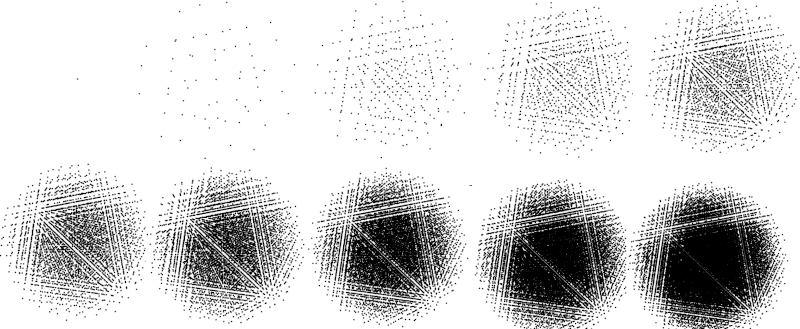
\includegraphics[scale=0.60]{e8to4dto3dpoints10shellslow.png}
    \caption{First 10 shells from E8 lattice to 4D ESQC to a 3D slice.}
    \label{e8to3dfirstshells}
\end{figure}

The notion of tiling spaces arises by considering each possible tiling that can be built on a specific CPS as a point in this space. Quantum mechanically, any possible tiling can be defined as a state, and instead, we work with the concept of Hilbert spaces. Thus, tiling spaces provide a robust framework for describing the geometric and quantum mechanical properties of the universe's expansion.

\subsection{Universe as a Growing Quasicrystal Hypothesis}

Our working hypothesis is that the universe is a growing quasicrystal. This is a simple heuristic model of the universe. Let us gather support for this idea and explore its consequences.


This model proposes an unconventional origin of the universe, diverging from the traditional Big Bang theory. It suggests that the universe began with the projection of a single point from a higher-dimensional lattice, such as the E8 root lattice. This initiated a sequence of point projections that sequentially constructed the universe's structure. This process, governed by a computational framework, unfolds step by step transitioning from one shell $N_{\text{E8}}(n)$ to the next $N_{\text{E8}}(n+1)$ and so forth. The number of points in each shell grows rapidly, with the first ten shells containing {240, 2160, 6720, 17520, 30240, 60480, 82560, 140400, 181680, 272160} points, respectively.  
The projection into a 4D quasicrystalline structure not only expands the universe but also intricately subdivides it internally, as points from newer shells intermingle with those from older shells, showcasing a complex process of growth and subdivision characteristic of the universe's early stages (see Figure \ref{fibchain} for a lower-dimensional illustration).
\begin{figure}[!h]
    \centering
    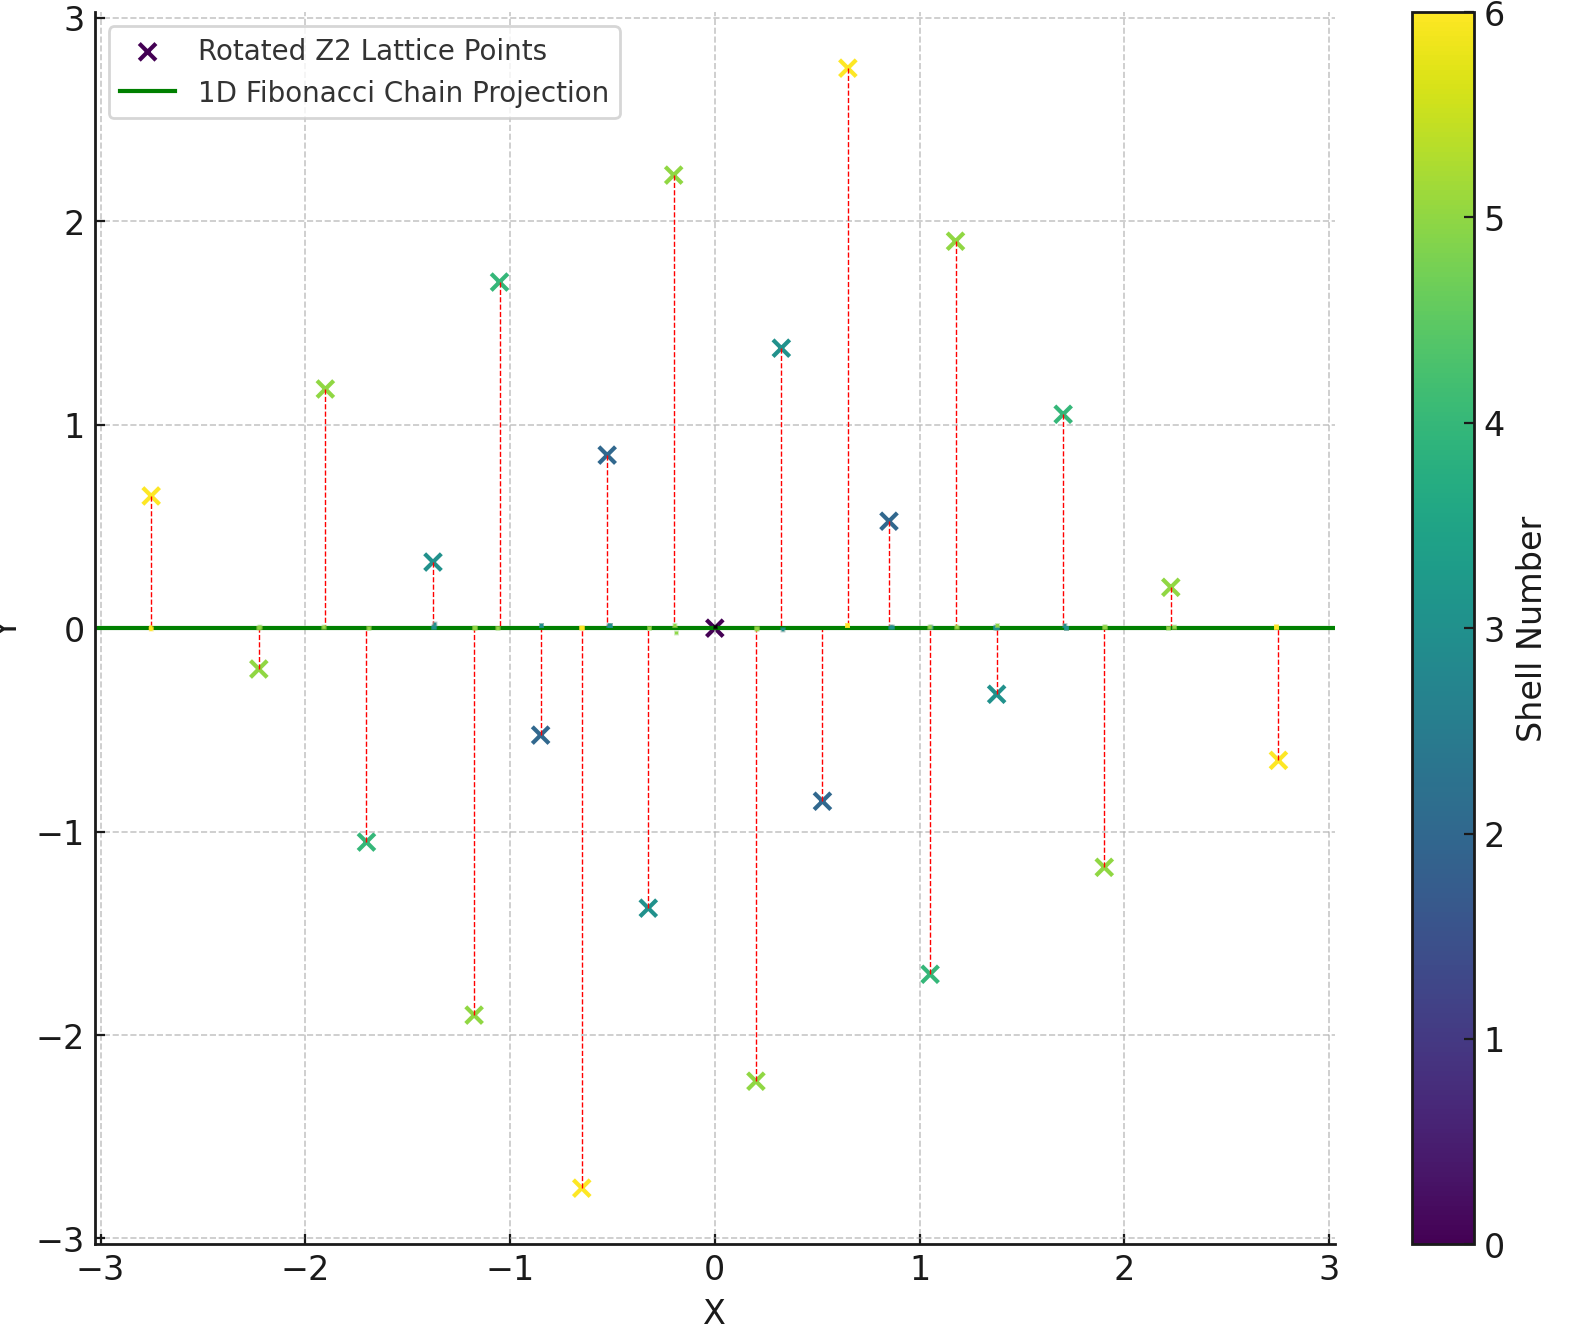
\includegraphics[scale=0.80]{Z2toFibChainGrowth1.png}
    \caption{A rotated Z2 being projected shell by shell with the color tracking the ordering. As this one dimensional universe expands, it also get new points inside the already projected region.}
    \label{fibchain}
\end{figure}

In this early stage, the universe consists of points, which are projections from the higher-dimensional root lattice. In the Lie algebra framework of modern gauge theories, these points represent fundamental particle states that form the Hilbert spaces of representations of the Lie algebra. At this stage, there is no scale or mass, and thus no distinction between particles, highlighting an analogy to the grand unification scale.

In condensed matter physics, a growing quasicrystal is associated with expanding Hilbert spaces. We can conjecture a similar process for the universe. As the universe grows, a burgeoning Hilbert space $\mathcal{H}_n$ emerges at each growth step $n$, reflecting the tiling spaces \cite{sadun2018} of potential quasicrystalline configurations. To address the different tiling configurations of quasicrystals, it is standard to consider the associated \( C^* \)-algebra structures \cite{Connes} and the notion of tiling spaces. This Hilbert space can be constructed as follows: Let $\mathcal{T}_n$ denote the set of all distinct tiling configurations at the $n$-th growth step, with each tiling configuration $T_n \in \mathcal{T}_n$ represented as a basis state $|T_n\rangle$ in $\mathcal{H}_n$. The growth process from step $n$ to $n+1$ can be expressed as:
\begin{align}
\mathcal{T}_n &\rightarrow \mathcal{T}_{n+1}, \\
\mathcal{H}_n &\rightarrow \mathcal{H}_{n+1}.
\end{align}

The wavefunction of the universe at the $n$-th growth step, $|\Psi_n\rangle \in \mathcal{H}_n$, can be written as a superposition of all possible tiling configurations:
\begin{equation}
|\Psi_n\rangle = \sum_{T_n \in \mathcal{T}_n} \alpha(T_n) |T_n\rangle,
\end{equation}
where $\alpha(T_n)$ are complex coefficients determined by the specific growth rules of the quasicrystal. As the universe grows, the wavefunction evolves to incorporate the new tiling configurations that emerge at each step, $|\Psi_n\rangle \rightarrow |\Psi_{n+1}\rangle$.

This growing Hilbert space structure suggests that the early universe may be viewed as a form of a quasicrystalline topological quantum computer, with quantum error-correcting codes (QECCs) inherently embedded \cite{Li:2023nkr}. At each growth step, a subspace $\mathcal{C}_n \subset \mathcal{H}_n$ can be identified, spanned by a set of wavefunctions ${|\Psi{n,[T]}\rangle}$ that exhibit local indistinguishability and recoverability properties \cite{Li:2023nkr}:
\begin{equation}
|\Psi_{n,[T]}\rangle = \sum_{g \in G_n} \beta(g T_n) |g T_n\rangle,
\end{equation}
where $[T]$ denotes an equivalence class of tiling configurations related by the symmetry group $G_n$, and $\beta(g T_n)$ are complex coefficients. The subspace $\mathcal{C}_n = \text{span}({|\Psi_{n,[T]}\rangle})$ can be interpreted as the code space of a QECC at the $n$-th growth step, capable of correcting errors in any local region of the quasicrystal. As the universe grows, the QECC evolves, $\mathcal{C}_n \rightarrow \mathcal{C}_{n+1}$.

This growing QECC structure provides a framework for understanding how quantum information can be encoded and protected within the geometry of a quasicrystalline universe. Notably, the Hilbert spaces associated with certain quasicrystals are isomorphic to the fusion Hilbert spaces that appear in topological quantum computing systems \cite{Amaral2022sy}. This establishes a connection between QECCs and topological quantum computation within the context of our working hypothesis of the growing quasicrystalline universe.

The emergence of this quasicrystalline structure and its associated Hilbert spaces in the early universe may have profound implications for the evolution of spacetime, matter, and quantum information processing. As the universe continues to grow and evolve, the interplay between the quasicrystalline geometry, QECCs, and topological quantum computation may guide the formation of large-scale cosmic structures and the emergence of complex phenomena. This heuristic model offers a novel perspective on the origin and evolution of the universe, connecting ideas from condensed matter physics, quantum information theory, and cosmology.



As the quasicrystalline universe evolves, phonons and phasons should emerge naturally due to the intrinsic properties of growing quasicrystals, even those composed of 'spacetime atoms.' Phonons correspond to collective vibrational modes of the tiling configurations, while phasons are associated with the rearrangement of the quasicrystalline structure without changing the overall energy. The presence of these quasiparticles is significant, as their dispersion relations lead to a form of the Friedmann equation (Equation \ref{phasonH2}), implying the establishment of standard expansion.

To incorporate phonons and phasons into our quantum description of tiling spaces, we introduce creation and annihilation operators acting on the Hilbert space $\mathcal{H}_n$ at each growth step. Let $a^{\dagger}_{k,n}$ and $a_{k,n}$ denote the creation and annihilation operators for a phonon with wave vector $k$ at the $n$-th growth step, satisfying the commutation relations:
\begin{equation}
[a_{k,n}, a^{\dagger}_{k',n}] = \delta_{k,k'}, \quad [a_{k,n}, a_{k',n}] = [a^{\dagger}_{k,n}, a^{\dagger}_{k',n}] = 0.
\end{equation}

Similarly, let $b^{\dagger}_{q,n}$ and $b_{q,n}$ denote the creation and annihilation operators for a phason with wave vector $q$ at the $n$-th growth step, satisfying similar commutation relations:
\begin{equation}
[b_{q,n}, b^{\dagger}_{q',n}] = \delta_{q,q'}, \quad [b_{q,n}, b_{q',n}] = [b^{\dagger}_{q,n}, b^{\dagger}_{q',n}] = 0.
\end{equation}
The phonon and phason operators commute with each other:
\begin{equation}
[a_{k,n}, b_{q,n}] = [a_{k,n}, b^{\dagger}_{q,n}] = [a^{\dagger}_{k,n}, b_{q,n}] = [a^{\dagger}_{k,n}, b^{\dagger}_{q,n}] = 0.
\end{equation}
Using these operators, we define phonon and phason excited states by acting on the tiling configuration states $|T_n\rangle$:
\begin{align}
|T_n; \{k\}_m; \{q\}_l\rangle &= a^{\dagger}_{k_1,n} \ldots a^{\dagger}_{k_m,n} b^{\dagger}_{q_1,n} \ldots b^{\dagger}_{q_l,n} |T_n\rangle,
\end{align}
where $\{k\}_m = \{k_1, \ldots, k_m\}$ and $\{q\}_l = \{q_1, \ldots, q_l\}$ characterize the $m$ phonons and $l$ phasons, respectively.

The growth of the quasicrystalline universe can be described in terms of the evolution of these excited states. As the universe grows from step $n$ to step $n+1$, the phonon and phason creation and annihilation operators evolve:
\begin{align}
a^{\dagger}_{k,n} &\rightarrow a^{\dagger}_{k,n+1}, \quad a_{k,n} \rightarrow a_{k,n+1}, \\
b^{\dagger}_{q,n} &\rightarrow b^{\dagger}_{q,n+1}, \quad b_{q,n} \rightarrow b_{q,n+1}.
\end{align}
The wavefunctions $|\Psi_n\rangle$ and $|\Psi_{n,[T]}\rangle$ can be expanded in terms of these excited states:
\begin{align}
|\Psi_n\rangle &= \sum_{T_n \in \mathcal{T}_n} \sum_{\{k\}, \{q\}} \alpha(T_n; \{k\}, \{q\}) |T_n; \{k\}; \{q\}\rangle, \\
|\Psi_{n,[T]}\rangle &= \sum_{g \in G_n} \sum_{\{k\}, \{q\}} \beta(g T_n; \{k\}, \{q\}) |g T_n; \{k\}; \{q\}\rangle,
\end{align}
where the coefficients $\alpha(T_n; \{k\}, \{q\})$ and $\beta(g T_n; \{k\}, \{q\})$ depend on both the tiling configurations and the phonon and phason excitations.


The emergence of phonons and phasons in the growing quasicrystalline universe has important implications for the properties of the corresponding quantum error-correcting codes. The presence of these excitations introduces additional degrees of freedom that may affect the error correction capabilities of the code. As discussed in the previous section, the dispersion relations of phonons and phasons lead to Friedmann-like equations describing the expansion of the universe, contributing to the energy density and exhibiting different behaviors in various phases of cosmological evolution.

In particular, the dispersion relation for phasons (Equation \ref{eq:phasonrelation}) includes an imaginary term that becomes significant at large wavelengths, leading to diffusive behavior, thereby excluding its contribution from the energy density. We can conjecture an early inflationary-like phase where this diffusive behavior of phasons marks the end of the inflationary phase and the emergence of matter \cite{modelsetemergence}. This transition signifies a shift from a universe dominated by phonon and phason expansion to a more complex interplay of matter, radiation, and spacetime dynamics, in the spirit of \cite{Barbour2003}. We propose that phonon and phason excitations can provide the seeds for composite matter formation.  
In this model, quasicrystal points act as point-particle excitations, forming composite particles such as hadrons. These excitations contribute to the radiation epoch spectrum, and as more composite matter emerges, the universe transitions to a matter-dominated epoch. As the universe expands, phonon and phason excitations may continue to influence its evolution.

\subsubsection{Tiling Spaces: From Discrete to Continuous}
While quantum field theory may be suitable for studying these transitions, most many-body systems, including quasicrystals and the universe, exist at finite temperatures. As a result, the equilibrium state of the system is described by a thermal density matrix, often involving mixed states. Consequently, conventional quantum field theory techniques may not be appropriate. The literature frequently employs effective field theory techniques to address these conditions. Here, we will describe tiling spaces using the probabilistic approach of \cite{BaakeGrimm}. Tiling spaces are defined by the continuous hull $X(\varLambda)$, which includes all translates of a point set $\varLambda$ in $\mathbb{R}^{d}$. This framework is typically applied to infinite quasicrystals, but to understand regimes where dynamics occur at scales much larger than the underlying spacing (potentially at the Planck scale), we expect to recover invariance under continuous translations in the tiling space.

A characteristic property of a point set in $\mathbb{R}^{d}$ is the average number of points per unit volume, and we are interested in the relative frequency $f^{r}$ of subsets or clusters of points, defined as the absolute frequency per unit volume over the density of the point set $\varLambda$. Various methods to compute this quantity can be found in the quasicrystal literature \cite{BaakeGrimm}. This will allow us to define a probabilistic measure in the tiling space.


These relative frequencies define an invariant probability measure on the set of tiling configurations $X_{0}(\varLambda)$, which consists of all tiling configurations with the origin as a point. For a non-empty finite cluster $P$, we define the cylinder set $Z_{P}$ containing all configurations with $P$ as a subcluster:
\begin{equation}
Z_{P}:=\{\varLambda'\in X_{0}(\varLambda)\mid P\subset\varLambda'\}.
\end{equation}
The measure of this cylinder set is given by the relative frequency:
\begin{equation}
\mu_{0}(Z_{P})=f_{\varLambda}^{r}(P).
\end{equation}

This measure extends to a positive measure on the entire tiling space $X(\varLambda)$ by standard arguments, using the \(\sigma\)-algebra generated by the cylinder sets.  
The invariant measure$\mu$ provides a robust framework to explore the statistical properties of quasicrystalline structures and their implications for cosmology. We can express the partition function as: 
\begin{align}
Z_{X} & =\sum_{\varLambda\in X(\varLambda)}\prod_{P\in\varLambda}f_{\varLambda}^{r}(P)=\sum_{\varLambda\in X(\varLambda)}\prod_{P\in\varLambda}\left(f_{\varLambda}^{r}\right)^{Nf_{\varLambda}^{r}}\nonumber \\
 & =\sum_{\varLambda\in X(\varLambda)}e^{N\sum_{P}f_{\varLambda}^{r}(P)\ln(f_{\varLambda}^{r}(P))}=\sum_{\varLambda\in X(\varLambda)}e^{-NI_{\varLambda}},
\end{align}
where $N$ is large, implying that the number of specific configurations
$P$ or clusters must approach its frequency. We introduce the information
entropy of the tiling space as 
\begin{equation}
I_{\varLambda}=-\sum_{P}f_{\varLambda}^{r}(P)\ln(f_{\varLambda}^{r}(P)).
\end{equation}

To connect this framework with a notion of energy density, we start
by calculating the emergent average energy $\langle E\rangle$ from
the partition function $Z$: 
\begin{equation}
\langle E\rangle=-\frac{\partial lnZ_{X}}{\partial\beta},
\end{equation}
where $\beta=N=\frac{1}{kT}$ is the inverse temperature. Note that
$N$ is playing the role of $\beta$. As the tiling space grows the
temperature lowers.

Given the volume $\eta$, the energy density $\rho$ is then: 
\begin{equation}
\rho=\frac{\langle E\rangle}{\eta}.
\end{equation}

This framework allows us to analyze the statistical properties of quasicrystalline structures and their implications for cosmology. The information entropy $I_{\varLambda}$ plays a crucial role in understanding the distribution and frequency of clusters within the tiling space, and the derived energy density connects this microscopic structure to macroscopic physical properties at large scales. With matter distributions, there are associated dispersion relations, which can lead to dynamics as we pointed out earlier.



Another aspect to consider is the self-similarity of quasicrystals. Quasicrystal point sets and associated tilings, while not retaining the discrete translational symmetry of the lattice in the projected space, exhibit new discrete symmetries such as scaling symmetry (self-similarity). This implies that the frequencies in a growing quasicrystal are dynamic and may oscillate.



Let us consider some suggestive interpretations of our working hypothesis of the universe as a growing quasicrystal. 

\subsubsection{Growth Dynamics in a Quasicrystalline Universe and Dark Energy}
This model incorporates two distinct types of growth, each playing a crucial role in the universe's evolution:

External Growth by Shell Projection:
The first type of growth occurs through the projection of new points from a higher-dimensional lattice onto our observable universe. This process can be visualized as the universe growing outward, shell by shell, from a central point. Each new shell introduces additional points, expanding the universe's structure.

Internal Growth through Subdivision and Rescaling:
The second type of growth is an internal process triggered by the introduction of matter, which naturally imposes a scale on the system. This scale can be aligned with the Planck scale, introducing minimum length and time scales. As new points are projected into the universe, they subdivide existing structures. To maintain consistency with the matter-imposed scale, the universe must undergo periodic rescaling.

To illustrate these growth processes, let's consider a simplified one-dimensional universe, the usual Fibonacci chain projected point by point:

Initial state: The universe begins with a single point and two tile lengths: short and long.

Second point: A new point arises. The original short tile becomes long, and a new short tile is introduced with the old long becoming a new long and a short.

Fourth point: With the addition of the fourth point, we now have three types of tiles. This illustrates the dynamic nature of the frequency distribution due to the asynchronicity between shell projections and the self-similarity requirements.

Fifth point: At this stage, we return to having two tile types, but at a different scale from the initial state.

If matter is defined based on the initial scale, the universe must rescale this new configuration to maintain consistency. The new long tile is rescaled to match the original long tile, and the same is done for the short tile.
This rescaling process is crucial for maintaining the consistency of matter within the growing quasicrystal structure. It allows for the preservation of local minimum distances between points if the rescaling is precisely timed after a certain number of points is projected.


Matter and observers are ultimately composed of points that are being replaced by new points projected from a higher dimension. This mechanism for dark energy can be modeled by assuming an energy constraint, leading to $\Lambda$ in Equations \ref{freedmanrela1} and \ref{freedmanrela2}.

The two distinct expansion processes may unfold differently in the early radiation-dominated epoch and the later matter-dominated epoch:
Growth due to the construction of the quasicrystal shell by shell from projections from a higher dimension.
Rescaling of internal subdivisions from points entering the quasicrystal from the projections, necessitated by matter fixing a scale.
This dual growth mechanism qualitatively addresses the Hubble tension.

\subsubsection{Phonons and Dark Matter}
In our quasicrystalline universe model, we can extend the analogy with solid-state physics to propose a novel explanation for dark matter. This approach leverages the concept of phonons—quantized modes of vibrations in a quasicrystal structure—and applies it to the spacetime quasicrystal of our model.

In this framework, spacetime itself is viewed as a quasicrystal, and phonons represent vibrational modes within this spacetime quasicrystal. These phonons, particularly those with long wavelengths that persist to later times, could potentially contribute to the dark matter component of the universe.
This concept draws a parallel with how phonons interact with electrons in solid-state physics. In solid-state systems, phonons can scatter electrons, influencing phenomena such as electrical resistance and superconductivity. The interaction Hamiltonian in solid-state physics typically takes the form:
\begin{equation}
H_{\text{int}} = g \sum_{q,k} (a_q + a_q^{\dagger}) c_{k+q}^{\dagger} c_k,
\end{equation}
where $a_q$ and $a_q^{\dagger}$ are phonon annihilation and creation operators, respectively, and $c_k$ and $c_{k+q}^{\dagger}$ are electron operators.

Extending this concept to our cosmological model, we can propose an interaction Lagrangian that couples spacetime phonons with ordinary matter (e.g., electrons):
\begin{equation}
\mathcal{L}_{\text{int}} = g_{ph} \sum_{q,k} (\phi_q + \phi_q^{\dagger}) \psi_{k+q}^{\dagger} \psi_k,
\end{equation}
where $\phi_q$ and $\phi_q^{\dagger}$ are the phonon fields, and $\psi_k$ and $\psi_{k+q}^{\dagger}$ are ordinary matter fields like electrons.

Dark Matter Candidate: These spacetime phonons, if weakly interacting, could serve as candidates for dark matter. They would influence the dynamics of ordinary matter while remaining largely undetectable through electromagnetic interactions. This is analogous to models where dark matter interacts with ordinary matter through new forces or mediators, modifying the dynamics of both dark matter and ordinary matter.
For instance, similar to dark photon interactions in some models, phonons in the spacetime quasicrystal could potentially scatter off nuclei, producing recoil signals that might be detectable in experiments designed to look for Weakly Interacting Massive Particles (WIMPs). Furthermore, the decay or annihilation of these phonons might produce standard model particles that could be detected by telescopes or neutrino detectors.
It's important to note that the quantitative details of this phonon-based dark matter model are still a work in progress. However, this approach offers a novel perspective on dark matter, grounded in the quasicrystalline structure of spacetime proposed by our model.
This phonon-based dark matter hypothesis not only provides a potential explanation for the nature of dark matter but also further illustrates the deep connections between solid-state physics and cosmology suggested by our quasicrystalline universe model.


\subsection{Implications of the Expanding Universe as a Growing Quasicrystal}

The hypothesis that the expanding universe is a growing quasicrystal has several significant implications for our understanding of cosmology:

1. \textbf{Elimination of the Inflation Scenario:} The necessity for an inflationary period may be obviated. The large number of tiles or points, $ N $, required for uniform distribution is achieved by construction through the imposition of a quasicrystalline structure. This uniformity, intrinsic to quasicrystals, provides a natural explanation for the observed large-scale homogeneity of the universe.

2. \textbf{Radiation Epoch:} Following the initial QECC construction phase, the universe enters a radiation-dominated epoch characterized by the emergence of phasons and phonons. These quasiparticles are analogous to relativistic matter and radiation, contributing to the early universe's dynamics. The presence of these quasiparticles can lead to unique dispersion relations influencing the energy density and expansion rate.

3. \textbf{Phason Contribution at Later Times:} At later times, as the number of points $N$ increases, phasons do not significantly contribute to the energy density. This is due to the dominance of a diffusive imaginary term in their dispersion relation at large wavelengths, effectively damping their influence on the universe's expansion.

4. \textbf{Matter and Long Wavelength Phonons:} Matter, along with long-wavelength massive phonons, continues to play a critical role in the universe's evolution. These components contribute to the overall energy density and can interact with ordinary matter, potentially acting as candidates for dark matter.

5. \textbf{Accelerated Expansion:} The universe's accelerated expansion can be explained by the internal rescaling mechanism driven by a fixed matter scale. This rescaling process results from the continuous projection and replacement of points within the quasicrystalline structure, analogous to the cosmological constant or dark energy driving the observed acceleration in the universe's expansion.

6. \textbf{States and Symmetries:} It is, however, questionable whether one can find exactly invariant states in a discrete space-time setting \cite{bojowald}. In the context of our quasicrystalline model, this suggests that the emergent large-scale symmetry is an approximation resulting from the statistical mechanics framework applied to the tiling space microstates. This leads to a partition function and energy densities that, in turn, give rise to Friedmann-like equations by imposing the Hubble law on the wavelength in the dispersion relation of propagating degrees of freedom.

Overall, this model provides a novel framework for understanding the universe's structure and dynamics, integrating concepts from condensed matter physics and cosmology to offer fresh perspectives on longstanding issues such as the Hubble tension and the nature of dark matter and dark energy.

-----

At this juncture, readers may question why projections occur, how the system determines which shells to project, and the nature of the computational framework underlying this higher dimensional lattice. They may also wonder if more lattices from higher dimensions are involved. These inquiries parallel conventional physics questions about the Big Bang, conservation laws, and the mechanisms underlying physical laws. Despite these profound questions, the hypothesis of a higher-dimensional framework introduces testable consequences for the cosmos—namely, the emergence of a quasicrystalline structure distinct from both continuous and traditional crystalline constructs.

If the cosmos possesses a quasicrystalline structure, this feature could potentially be identified using techniques similar to those employed in materials science for detecting crystalline arrangements. The structural nature of a material—whether crystalline, quasicrystalline, or amorphous—is revealed through distinctive diffraction patterns. In the lab, such patterns are commonly produced through electron diffraction, where an electron beam interacts with the material. The resultant diffraction pattern, which provides detailed information on atomic spacing and structure, is then recorded. The presence of definitive Bragg peaks within these patterns indicates constructive interference from regular atomic planes, revealing the material's symmetry and structure.

Applying this concept to a cosmic scale, one might consider the cosmic microwave background (CMB) radiation as a macroscopic "diffraction pattern" reflecting the universe's structure. The CMB, a relic radiation from the Big Bang, offers a primordial snapshot of the universe from 380,000 years after its inception, containing valuable structural and compositional data from that era. Detailed examination of temperature and polarization fluctuations within the CMB, as captured by observatories like the Planck satellite, allows researchers to piece together the universe's large-scale structure.

In a theoretical model positing quasicrystalline symmetry in the universe, this analysis would involve searching the CMB data for Bragg-like peaks—specific intensity points revealing an ordered pattern characteristic of quasicrystalline structures. Identifying such patterns would profoundly transform our understanding of the cosmic expanse and bridge celestial phenomena with quantum-scale observations in condensed matter physics.

\section{Discussion}
\label{sec:conclusion}

In this paper, we have expanded the interpretation of the wave function beyond its traditional role in estimating a particle's position probability. By exploring the Schr{\"o}dinger equation for a particle in a box with time-dependent boundaries and introducing a constraint that bridges microscale and macroscale quantities, we have derived an equation that bears a structural resemblance to the Friedmann equation. This development could be instrumental in addressing pivotal cosmological challenges, such as the Hubble tension. This tension arises due to observed discrepancies in the measurement of the universe's expansion rate, as denoted by the Hubble constant $H_0$. Notably, $H_0$ shows differing values when measured in the early universe—particularly via the CMB, indicating a slower expansion rate—compared to measurements from the late universe using supernovae and Cepheid variables, which suggest a faster expansion rate. Such variations point to a potential gap in our current understanding of the universe's expansion trajectory.

Furthermore, we have hypothesized a novel heuristic model of the expanding universe conceptualized as a quasicrystalline projection from a higher-dimensional lattice. The inherent properties of quasicrystals, which resonate with cosmological principles, offer promising insights into the dynamics of the cosmic scale parameter. Our approach introduces a fresh perspective on comprehending the universe's structure and its expansion, with a specific focus on unraveling the Hubble tension, dark energy, and dark matter. In our model, the universe's scale parameter is envisioned as a function of both the non-linear increase in points from projections from a higher-dimensional lattice and the rescaling of spaces inside the matter content of the universe with new points coming to the projected tiling space. The model provides a phase pre-inflation with quantum error correction, bypassing the inflation phase, and transitioning to a phase dominated by propagating phasons, phonons, and radiation. Subsequently, it evolves to a phase characterized by the emergence of matter in the limit of very large number of tiles, culminating in a later phase with two kinds of expansion engines due to the projections. Long-wavelength massive phonons arise as candidates for dark matter.

A potential critique of this model could be the apparent contradiction between the continuous symmetry observed in the universe and the discrete nature of a quasicrystalline structure. This critique can be addressed by noting that quasicrystals give rise to tiling spaces that exhibit continuous symmetry on very large scales. We introduced a statistical mechanics framework to show how this can occur, using a probabilistic measure for tiling space microstates, which leads to a partition function and energy densities. The Friedmann-like equations arise by imposing the Hubble law on the wavelength in the dispersion relation of propagating degrees of freedom.

To fully realize the potential of this approach, further detailed analysis is required. This will involve rigorously developing the quantitative model and enhancing its predictive power, thereby contributing significantly to our understanding of the universe's expansion and its underlying code structure.




%\section*{Acknowledgments}
%This was was supported in part by......
%\section{Acknowledgements}


%Bibliography
%\bibliographystyle{unsrt}  
%\bibliography{references}  


\begin{thebibliography}{999}
%
\bibitem{Verlinde2011}
    Verlinde, E. On the origin of gravity and the laws of Newton. J. High Energ. Phys. 2011, 29 (2011). 	
\bibitem{Rovelli-Vidotto-Book} 
	Rovelli, C., Vidotto, F.:
	Covariant Loop Quantum Gravity.
	  Cambridge University Press  1 edition, (2014).

\bibitem{stringbook1} 
 	Green, M. B., Schwarz, J. H., Witten, E.: Superstring Theory, Vol. I and Vol. II, Cambridge University Press (1988).

\bibitem{Kiefer}
    Kiefer, C. Quantum Gravity: Third Edition. (OUP Oxford,2012)
    
\bibitem{Rovelli1998} 
  Rovelli, C. Loop Quantum Gravity. Living Rev. Relativ. 1, 1 (1998). arXiv:gr-qc/9710008.

\bibitem{Tahim2009} 
    Tahim, M. O., Landim, R. R., Almeida, C. A. S. Spacetime as a deformable solid. Modern Physics Letters A. Vol. 24, No. 15, pp. 1209-1217 (2009).
    arXiv:0705.4120 [gr-qc].
    
\bibitem{Amaral:2023mgf}
    M.~Amaral, R.~Clawson and K.~Irwin,
    Quasicrystalline Spin Foam with Matter: Definitions and Examples,
    [arXiv:2306.01964 [gr-qc]].

\bibitem{modelsetemergence} 
  Amaral, M.; Fang, F.; Aschheim, R.; Irwin, K. On the Emergence of Spacetime and Matter from Model Sets. Preprints 2021, 2021110359. https://doi.org/10.20944/preprints202111.0359.v2
  
\bibitem{lawsofnature}
    Gaspar, Y., Tambor, P. The Laws of Nature and the Problems of Modern Cosmology. Found Sci (2023). https://doi.org/10.1007/s10699-023-09904-1
        
\bibitem{hubbletension}
    Huterer, D. Hubble tension. Eur. Phys. J. Plus 138, 1004 (2023). https://doi.org/10.1140/epjp/s13360-023-04591-0
        
\bibitem{hubble}
    Riess, A., \& Anand, G. (2024). Webb and Hubble Affirm Universe’s Expansion Rate, Puzzle Persists. The Astrophysical Journal Letters.
    
\bibitem{bojowald}
     Martin Bojowald 2015 Rep. Prog. Phys. 78 023901
     DOI 10.1088/0034-4885/78/2/023901
    
\bibitem{Kuzmichev}
     Kuzmichev, V.E., Kuzmichev, V.V. The Hubble tension from the standpoint of quantum cosmology. Eur. Phys. J. C 84, 121 (2024). https://doi.org/10.1140/epjc/s10052-024-12490-6
     
\bibitem{Cooney}
    K. Cooney. The infinite potential well with moving walls. arXiv:1703.05282 [quant-ph], (2017).
    
\bibitem{francisco}
    Francisco Ricardo Torres Arvizu et al, On the energy density in quantum mechanics. Phys. Scr. 98, 125015, (2023).

\bibitem{Koehn:2012red}
    M.~Koehn,
    Solutions of the Klein-Gordon equation in an infinite square-well potential with a moving wall,
    EPL \textbf{100}, no.6, 60008 (2012)
    [arXiv:1301.0436 [math-ph]].

\bibitem{Baggioli:2020haa}
    M.~Baggioli and M.~Landry,
    Effective Field Theory for Quasicrystals and Phasons Dynamics,
    SciPost Phys. \textbf{9}, no.5, 062 (2020)
    [arXiv:2008.05339 [hep-th]].

\bibitem{Lubensky}
    T. C. Lubensky, Sriram Ramaswamy, and John Toner, Hydrodynamics of icosahedral quasicrystals. Phys. Rev. B 32, 7444, (1985).

\bibitem{BaakeGrimm} 
 	Baake, M., Grimm, U. Aperiodic Order, Cambridge University Press, (2013).

\bibitem{ElserSloane1987}
    Elser, V. and Sloane, N. J. A., A highly symmetric four-dimensional quasicrystal, J. Phys. A 20, 6161, (1987).

\bibitem{ConwaySloane1988}
     Conway, J. H. and Sloane, N. J. A. Sphere Packins Lorricer and Groups (Berlin: Springer) (1988).

\bibitem{sadun2018}
	Sadun, L.: Tilings, tiling spaces and topology, Philosophical Magazine 86, 875-881, (2006). 

\bibitem{Connes} 
  Connes, A.: Non-commutative geometry, Boston, MA: Academic Press, (1994).

\bibitem{Li:2023nkr}
    Z.~Li and L.~Boyle,
    ``The Penrose Tiling is a Quantum Error-Correcting Code,''
    [arXiv:2311.13040 [quant-ph]].
    
\bibitem{Amaral2022sy}
    Amaral, M.; Chester, D.; Fang, F.; Irwin, K. Exploiting Anyonic Behavior of Quasicrystals for Topological Quantum Computing. Symmetry 2022, 14, 1780. https://doi.org/10.3390/sym14091780
    
\bibitem{Barbour2003} 
    Barbour, J. Class. Quantum Grav. 20, 1543. (2003)
    https://doi.org/10.1088/0264-9381/20/8/310
    
\bibitem{Fabbrichesi2020}
    M.~Fabbrichesi, E.~Gabrielli, and G.~Lanfranchi,
    ``The Physics of the Dark Photon: A Primer,''
    SpringerBriefs in Physics, Springer, Cham (2020),
    doi:10.1007/978-3-030-62519-1.



\end{thebibliography}

\end{document}
